\documentclass[12pt,a4paper]{article}

% ============================================
% PACKAGES
% ============================================
\usepackage[utf8]{inputenc}
\usepackage[T1]{fontenc}
\usepackage[english]{babel}
\usepackage{geometry}
\usepackage{graphicx}
\usepackage{xcolor}
\usepackage{tikz}
\usepackage{booktabs}
\usepackage{longtable}
\usepackage{array}
\usepackage{multirow}
\usepackage{fancyhdr}
\usepackage{titlesec}
\usepackage{hyperref}
\usepackage{listings}
\usepackage{float}
\usepackage{tcolorbox}

% TikZ libraries
\usetikzlibrary{shapes, arrows, positioning, calc, fit, backgrounds, shadows}

% ============================================
% PAGE SETUP
% ============================================
\geometry{
    left=2cm,
    right=2cm,
    top=2.5cm,
    bottom=2.5cm
}

% ============================================
% COLORS
% ============================================
\definecolor{primaryblue}{RGB}{0, 82, 147}
\definecolor{secondaryblue}{RGB}{100, 149, 237}
\definecolor{entitycolor}{RGB}{173, 216, 230}
\definecolor{pkcolor}{RGB}{255, 215, 0}
\definecolor{fkcolor}{RGB}{144, 238, 144}
\definecolor{relationcolor}{RGB}{255, 99, 71}
\definecolor{hdfscolor}{RGB}{255, 182, 108}
\definecolor{postgrescolor}{RGB}{135, 206, 250}

% ============================================
% HEADER/FOOTER
% ============================================
\pagestyle{fancy}
\fancyhf{}
\fancyhead[L]{\textcolor{primaryblue}{\textbf{Procurement Data Pipeline}}}
\fancyhead[R]{\textcolor{primaryblue}{Data Models - UML \& MCD/MLD}}
\fancyfoot[C]{\thepage}
\renewcommand{\headrulewidth}{0.5pt}
\renewcommand{\footrulewidth}{0.5pt}

% ============================================
% TITLE FORMATTING
% ============================================
\titleformat{\section}
{\color{primaryblue}\normalfont\Large\bfseries}
{\thesection}{1em}{}

\titleformat{\subsection}
{\color{secondaryblue}\normalfont\large\bfseries}
{\thesubsection}{1em}{}

% ============================================
% HYPERLINKS
% ============================================
\hypersetup{
    colorlinks=true,
    linkcolor=primaryblue,
    urlcolor=primaryblue,
    citecolor=primaryblue
}

% ============================================
% DOCUMENT START
% ============================================
\begin{document}

% ============================================
% TITLE PAGE
% ============================================
\begin{titlepage}
    \centering
    \vspace*{2cm}
    
    {\Huge\textcolor{primaryblue}{\textbf{Procurement Data Pipeline}}}
    
    \vspace{0.5cm}
    
    {\Large\textcolor{secondaryblue}{Data Modeling Documentation}}
    
    \vspace{1.5cm}
    
    {\LARGE\textbf{UML Class Diagram \& MCD/MLD}}
    
    \vspace{2cm}
    
    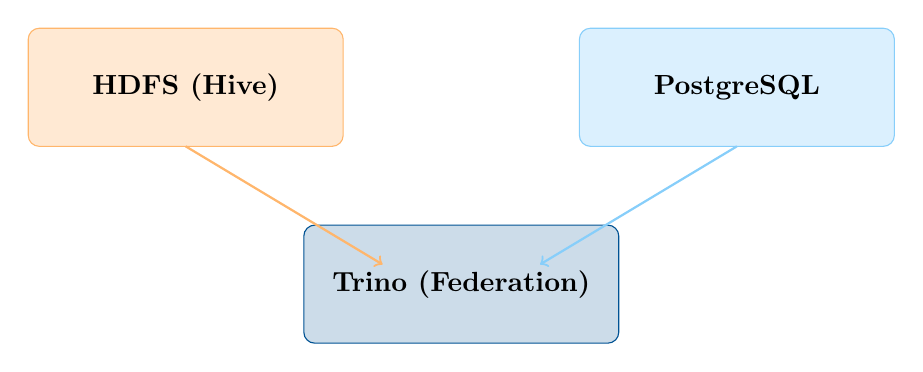
\begin{tikzpicture}
        % HDFS Box
        \node[draw=hdfscolor, fill=hdfscolor!30, rounded corners, minimum width=4cm, minimum height=1.5cm] at (-3.5,0) {
            \textbf{HDFS (Hive)}
        };
        
        % PostgreSQL Box
        \node[draw=postgrescolor, fill=postgrescolor!30, rounded corners, minimum width=4cm, minimum height=1.5cm] at (3.5,0) {
            \textbf{PostgreSQL}
        };
        
        % Trino Box
        \node[draw=primaryblue, fill=primaryblue!20, rounded corners, minimum width=4cm, minimum height=1.5cm] at (0,-2.5) {
            \textbf{Trino (Federation)}
        };
        
        % Arrows
        \draw[->, thick, hdfscolor] (-3.5,-0.75) -- (-1,-2.25);
        \draw[->, thick, postgrescolor] (3.5,-0.75) -- (1,-2.25);
    \end{tikzpicture}
    
    \vspace{2cm}
    
    {\large\textbf{Authors:}}\\
    \vspace{0.3cm}
    {\large SAID Salma \& TAMZIRT Mohamed}
    
    \vspace{1cm}
    
    {\large\textbf{Data Engineering Department}}
    
    \vspace{0.5cm}
    
    {\large December 2025}
    
\end{titlepage}

% ============================================
% TABLE OF CONTENTS
% ============================================
\tableofcontents
\newpage

% ============================================
% SECTION 1: UML CLASS DIAGRAM
% ============================================
\section{UML Class Diagram}

\subsection{Overview}

The UML Class Diagram represents the object-oriented view of the procurement data pipeline entities. It shows the classes, their attributes, methods, and relationships.

\subsection{Class Diagram}

\begin{figure}[H]
\centering
\resizebox{\textwidth}{!}{
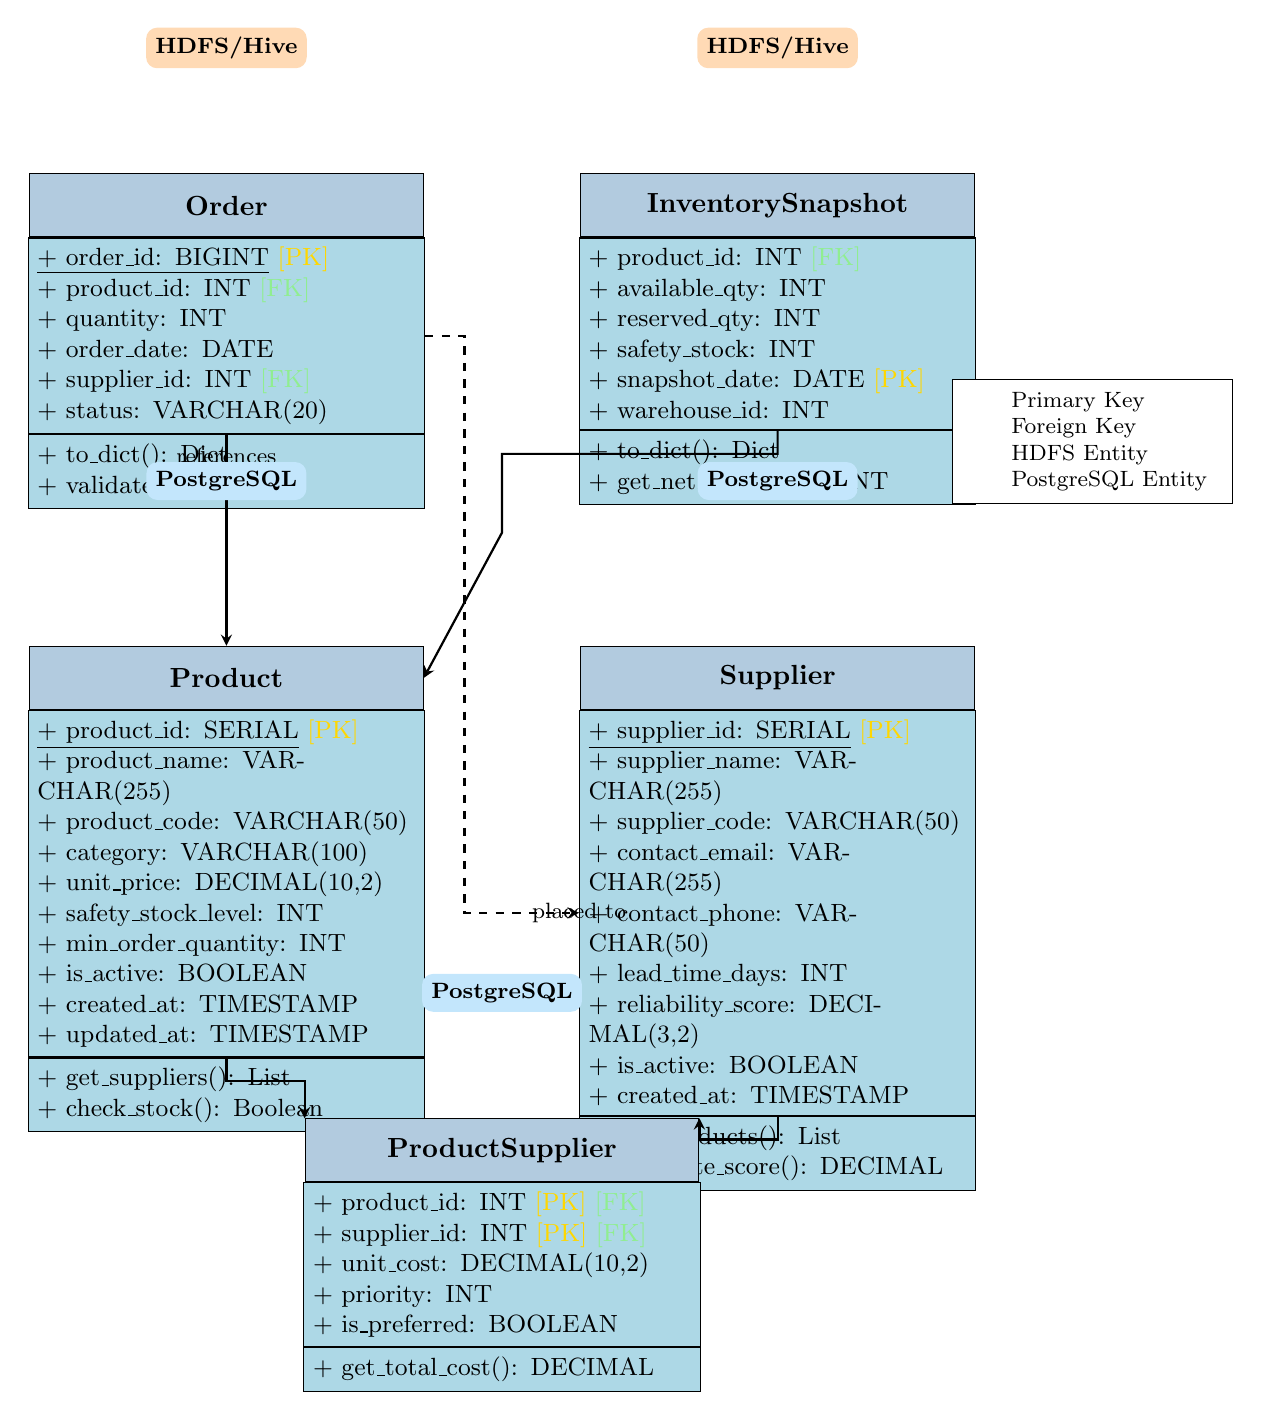
\begin{tikzpicture}[
    class/.style={
        rectangle, draw=black, fill=entitycolor, 
        minimum width=5cm, text width=4.8cm,
        font=\small
    },
    classname/.style={
        rectangle, draw=black, fill=primaryblue!30,
        minimum width=5cm, minimum height=0.8cm,
        font=\bfseries
    },
    arrow/.style={->, >=stealth, thick}
]

% =====================================================
% ORDER CLASS (HDFS)
% =====================================================
\node[classname] (order_name) at (0, 8) {Order};
\node[class, below=0pt of order_name, anchor=north] (order_attr) {
    \underline{+ order\_id: BIGINT} \textcolor{pkcolor}{[PK]}\\
    + product\_id: INT \textcolor{fkcolor}{[FK]}\\
    + quantity: INT\\
    + order\_date: DATE\\
    + supplier\_id: INT \textcolor{fkcolor}{[FK]}\\
    + status: VARCHAR(20)
};
\node[class, below=0pt of order_attr, anchor=north] (order_methods) {
    + to\_dict(): Dict\\
    + validate(): Boolean
};

% =====================================================
% INVENTORY SNAPSHOT CLASS (HDFS)
% =====================================================
\node[classname] (inv_name) at (7, 8) {InventorySnapshot};
\node[class, below=0pt of inv_name, anchor=north] (inv_attr) {
    + product\_id: INT \textcolor{fkcolor}{[FK]}\\
    + available\_qty: INT\\
    + reserved\_qty: INT\\
    + safety\_stock: INT\\
    + snapshot\_date: DATE \textcolor{pkcolor}{[PK]}\\
    + warehouse\_id: INT
};
\node[class, below=0pt of inv_attr, anchor=north] (inv_methods) {
    + to\_dict(): Dict\\
    + get\_net\_available(): INT
};

% =====================================================
% PRODUCT CLASS (PostgreSQL)
% =====================================================
\node[classname] (prod_name) at (0, 2) {Product};
\node[class, below=0pt of prod_name, anchor=north] (prod_attr) {
    \underline{+ product\_id: SERIAL} \textcolor{pkcolor}{[PK]}\\
    + product\_name: VARCHAR(255)\\
    + product\_code: VARCHAR(50)\\
    + category: VARCHAR(100)\\
    + unit\_price: DECIMAL(10,2)\\
    + safety\_stock\_level: INT\\
    + min\_order\_quantity: INT\\
    + is\_active: BOOLEAN\\
    + created\_at: TIMESTAMP\\
    + updated\_at: TIMESTAMP
};
\node[class, below=0pt of prod_attr, anchor=north] (prod_methods) {
    + get\_suppliers(): List\\
    + check\_stock(): Boolean
};

% =====================================================
% SUPPLIER CLASS (PostgreSQL)
% =====================================================
\node[classname] (sup_name) at (7, 2) {Supplier};
\node[class, below=0pt of sup_name, anchor=north] (sup_attr) {
    \underline{+ supplier\_id: SERIAL} \textcolor{pkcolor}{[PK]}\\
    + supplier\_name: VARCHAR(255)\\
    + supplier\_code: VARCHAR(50)\\
    + contact\_email: VARCHAR(255)\\
    + contact\_phone: VARCHAR(50)\\
    + lead\_time\_days: INT\\
    + reliability\_score: DECIMAL(3,2)\\
    + is\_active: BOOLEAN\\
    + created\_at: TIMESTAMP
};
\node[class, below=0pt of sup_attr, anchor=north] (sup_methods) {
    + get\_products(): List\\
    + calculate\_score(): DECIMAL
};

% =====================================================
% PRODUCT_SUPPLIER ASSOCIATION CLASS (PostgreSQL)
% =====================================================
\node[classname] (ps_name) at (3.5, -4) {ProductSupplier};
\node[class, below=0pt of ps_name, anchor=north] (ps_attr) {
    + product\_id: INT \textcolor{pkcolor}{[PK]} \textcolor{fkcolor}{[FK]}\\
    + supplier\_id: INT \textcolor{pkcolor}{[PK]} \textcolor{fkcolor}{[FK]}\\
    + unit\_cost: DECIMAL(10,2)\\
    + priority: INT\\
    + is\_preferred: BOOLEAN
};
\node[class, below=0pt of ps_attr, anchor=north] (ps_methods) {
    + get\_total\_cost(): DECIMAL
};

% =====================================================
% RELATIONSHIPS
% =====================================================

% Order -> Product (many-to-one)
\draw[arrow, thick] (order_attr.south) -- ++(0,-0.5) -| node[pos=0.25, above, font=\footnotesize] {references} (prod_name.north);

% Order -> Supplier (many-to-one)
\draw[arrow, thick, dashed] (order_attr.east) -- ++(0.5,0) |- node[pos=0.75, right, font=\footnotesize] {placed to} (sup_attr.west);

% InventorySnapshot -> Product (many-to-one)
\draw[arrow, thick] (inv_attr.south) -- ++(0,-0.3) -- ++(-3.5,0) -- ++(0,-1) -- (prod_name.east);

% Product -> ProductSupplier (one-to-many)
\draw[arrow, thick] (prod_attr.south) -- ++(0,-0.3) -| (ps_name.north west);

% Supplier -> ProductSupplier (one-to-many)
\draw[arrow, thick] (sup_attr.south) -- ++(0,-0.3) -| (ps_name.north east);

% Legend
\node[draw, fill=white, font=\footnotesize] at (11, 5) {
    \begin{tabular}{cl}
        \textcolor{pkcolor}{$\blacksquare$} & Primary Key\\
        \textcolor{fkcolor}{$\blacksquare$} & Foreign Key\\
        \textcolor{hdfscolor}{$\blacksquare$} & HDFS Entity\\
        \textcolor{postgrescolor}{$\blacksquare$} & PostgreSQL Entity
    \end{tabular}
};

% Storage indicators
\node[fill=hdfscolor!50, rounded corners, font=\footnotesize\bfseries] at (0, 10) {HDFS/Hive};
\node[fill=hdfscolor!50, rounded corners, font=\footnotesize\bfseries] at (7, 10) {HDFS/Hive};
\node[fill=postgrescolor!50, rounded corners, font=\footnotesize\bfseries] at (0, 4.5) {PostgreSQL};
\node[fill=postgrescolor!50, rounded corners, font=\footnotesize\bfseries] at (7, 4.5) {PostgreSQL};
\node[fill=postgrescolor!50, rounded corners, font=\footnotesize\bfseries] at (3.5, -2) {PostgreSQL};

\end{tikzpicture}
}
\caption{UML Class Diagram - Procurement Data Pipeline}
\label{fig:uml}
\end{figure}

\subsection{Relationships Description}

\begin{table}[H]
\centering
\begin{tabular}{|l|l|l|p{5cm}|}
\hline
\rowcolor{primaryblue!20}
\textbf{Source} & \textbf{Target} & \textbf{Cardinality} & \textbf{Description} \\
\hline
Order & Product & N:1 & Each order references one product \\
\hline
Order & Supplier & N:1 & Each order is placed to one supplier \\
\hline
InventorySnapshot & Product & N:1 & Each snapshot is for one product \\
\hline
Product & ProductSupplier & 1:N & A product can have multiple suppliers \\
\hline
Supplier & ProductSupplier & 1:N & A supplier can provide multiple products \\
\hline
\end{tabular}
\caption{UML Relationships}
\end{table}

\newpage

% ============================================
% SECTION 2: MCD (Modèle Conceptuel de Données)
% ============================================
\section{MCD - Modèle Conceptuel de Données}

\subsection{Overview}

The MCD (Conceptual Data Model) represents a high-level, technology-agnostic view of the data entities and their relationships using the Entity-Relationship (ER) notation.

\subsection{Entity-Relationship Diagram}

\begin{figure}[H]
\centering
\resizebox{\textwidth}{!}{
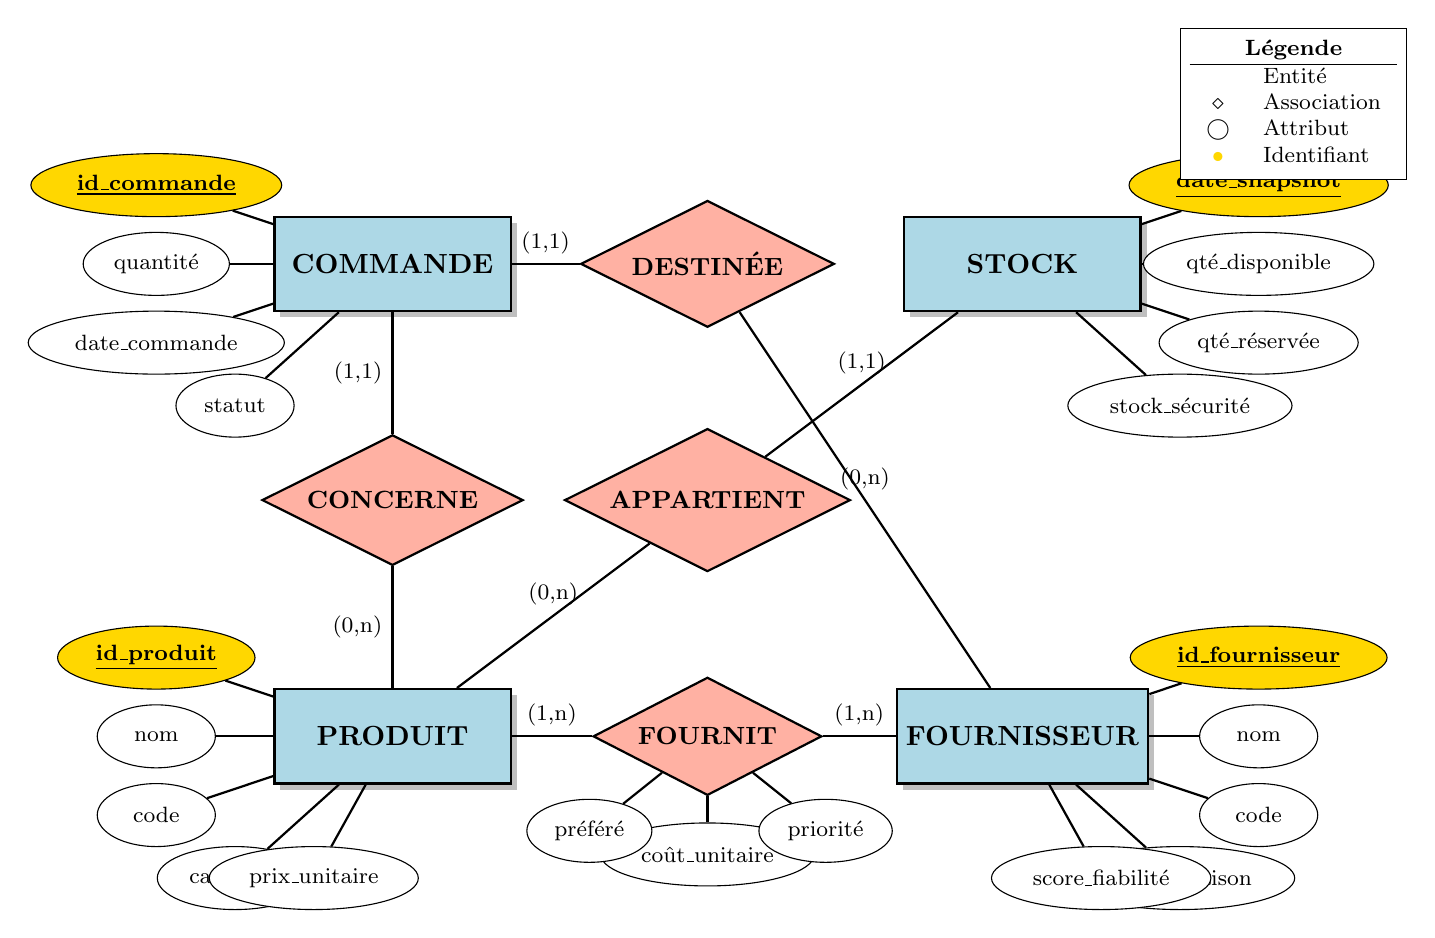
\begin{tikzpicture}[
    entity/.style={
        rectangle, draw=black, fill=entitycolor, 
        minimum width=3cm, minimum height=1.2cm,
        font=\bfseries, thick, drop shadow
    },
    relationship/.style={
        diamond, draw=black, fill=relationcolor!50,
        minimum width=2.5cm, minimum height=1.5cm,
        font=\bfseries\small, thick, aspect=2
    },
    attribute/.style={
        ellipse, draw=black, fill=white,
        minimum width=1.5cm, minimum height=0.8cm,
        font=\footnotesize
    },
    pk/.style={
        ellipse, draw=black, fill=pkcolor,
        minimum width=1.5cm, minimum height=0.8cm,
        font=\footnotesize\bfseries
    },
    line/.style={thick}
]

% =====================================================
% ENTITIES
% =====================================================

% PRODUCT Entity
\node[entity] (product) at (0, 0) {PRODUIT};

% SUPPLIER Entity
\node[entity] (supplier) at (8, 0) {FOURNISSEUR};

% ORDER Entity
\node[entity] (order) at (0, 6) {COMMANDE};

% INVENTORY Entity
\node[entity] (inventory) at (8, 6) {STOCK};

% =====================================================
% RELATIONSHIPS
% =====================================================

% Product -- Supplier (N:M via FOURNIT)
\node[relationship] (fournit) at (4, 0) {FOURNIT};

% Order -- Product (N:1 via CONCERNE)
\node[relationship] (concerne) at (0, 3) {CONCERNE};

% Order -- Supplier (N:1 via DESTINEE)
\node[relationship] (destinee) at (4, 6) {DESTINÉE};

% Inventory -- Product (N:1 via APPARTIENT)
\node[relationship] (appartient) at (4, 3) {APPARTIENT};

% =====================================================
% ATTRIBUTES - PRODUCT
% =====================================================
\node[pk] (prod_id) at (-3, 1) {\underline{id\_produit}};
\node[attribute] (prod_name) at (-3, 0) {nom};
\node[attribute] (prod_code) at (-3, -1) {code};
\node[attribute] (prod_cat) at (-2, -1.8) {catégorie};
\node[attribute] (prod_price) at (-1, -1.8) {prix\_unitaire};

\draw[line] (product) -- (prod_id);
\draw[line] (product) -- (prod_name);
\draw[line] (product) -- (prod_code);
\draw[line] (product) -- (prod_cat);
\draw[line] (product) -- (prod_price);

% =====================================================
% ATTRIBUTES - SUPPLIER
% =====================================================
\node[pk] (sup_id) at (11, 1) {\underline{id\_fournisseur}};
\node[attribute] (sup_name) at (11, 0) {nom};
\node[attribute] (sup_code) at (11, -1) {code};
\node[attribute] (sup_lead) at (10, -1.8) {délai\_livraison};
\node[attribute] (sup_score) at (9, -1.8) {score\_fiabilité};

\draw[line] (supplier) -- (sup_id);
\draw[line] (supplier) -- (sup_name);
\draw[line] (supplier) -- (sup_code);
\draw[line] (supplier) -- (sup_lead);
\draw[line] (supplier) -- (sup_score);

% =====================================================
% ATTRIBUTES - ORDER
% =====================================================
\node[pk] (ord_id) at (-3, 7) {\underline{id\_commande}};
\node[attribute] (ord_qty) at (-3, 6) {quantité};
\node[attribute] (ord_date) at (-3, 5) {date\_commande};
\node[attribute] (ord_status) at (-2, 4.2) {statut};

\draw[line] (order) -- (ord_id);
\draw[line] (order) -- (ord_qty);
\draw[line] (order) -- (ord_date);
\draw[line] (order) -- (ord_status);

% =====================================================
% ATTRIBUTES - INVENTORY
% =====================================================
\node[pk] (inv_date) at (11, 7) {\underline{date\_snapshot}};
\node[attribute] (inv_avail) at (11, 6) {qté\_disponible};
\node[attribute] (inv_res) at (11, 5) {qté\_réservée};
\node[attribute] (inv_safe) at (10, 4.2) {stock\_sécurité};

\draw[line] (inventory) -- (inv_date);
\draw[line] (inventory) -- (inv_avail);
\draw[line] (inventory) -- (inv_res);
\draw[line] (inventory) -- (inv_safe);

% =====================================================
% ATTRIBUTES - FOURNIT (Relationship attributes)
% =====================================================
\node[attribute] (f_cost) at (4, -1.5) {coût\_unitaire};
\node[attribute] (f_prio) at (5.5, -1.2) {priorité};
\node[attribute] (f_pref) at (2.5, -1.2) {préféré};

\draw[line] (fournit) -- (f_cost);
\draw[line] (fournit) -- (f_prio);
\draw[line] (fournit) -- (f_pref);

% =====================================================
% CONNECTIONS
% =====================================================

% Product -- Fournit -- Supplier
\draw[line] (product) -- node[above, font=\footnotesize] {(1,n)} (fournit);
\draw[line] (fournit) -- node[above, font=\footnotesize] {(1,n)} (supplier);

% Order -- Concerne -- Product
\draw[line] (order) -- node[left, font=\footnotesize] {(1,1)} (concerne);
\draw[line] (concerne) -- node[left, font=\footnotesize] {(0,n)} (product);

% Order -- Destinee -- Supplier
\draw[line] (order) -- node[above, font=\footnotesize] {(1,1)} (destinee);
\draw[line] (destinee) -- node[above, font=\footnotesize] {(0,n)} (supplier);

% Inventory -- Appartient -- Product
\draw[line] (inventory) -- node[above, font=\footnotesize] {(1,1)} (appartient);
\draw[line] (appartient) -- node[above, font=\footnotesize] {(0,n)} (product);

% Legend
\node[draw, fill=white, font=\footnotesize, anchor=north west] at (10, 9) {
    \begin{tabular}{cl}
        \multicolumn{2}{c}{\textbf{Légende}}\\
        \hline
        $\square$ & Entité\\
        $\diamond$ & Association\\
        $\bigcirc$ & Attribut\\
        \textcolor{pkcolor}{$\bullet$} & Identifiant\\
    \end{tabular}
};

\end{tikzpicture}
}
\caption{MCD - Modèle Conceptuel de Données}
\label{fig:mcd}
\end{figure}

\subsection{Règles de Gestion}

\begin{enumerate}
    \item Une \textbf{COMMANDE} concerne un et un seul \textbf{PRODUIT}
    \item Une \textbf{COMMANDE} est destinée à un et un seul \textbf{FOURNISSEUR}
    \item Un \textbf{PRODUIT} peut être fourni par plusieurs \textbf{FOURNISSEURS}
    \item Un \textbf{FOURNISSEUR} peut fournir plusieurs \textbf{PRODUITS}
    \item Un \textbf{STOCK} (snapshot) appartient à un et un seul \textbf{PRODUIT}
    \item Un \textbf{PRODUIT} peut avoir plusieurs snapshots de \textbf{STOCK}
\end{enumerate}

\newpage

% ============================================
% SECTION 3: MLD (Modèle Logique de Données)
% ============================================
\section{MLD - Modèle Logique de Données}

\subsection{Overview}

The MLD (Logical Data Model) represents the database-ready schema derived from the MCD. It includes primary keys, foreign keys, and data types.

\subsection{Relational Schema}

\begin{figure}[H]
\centering
\resizebox{\textwidth}{!}{
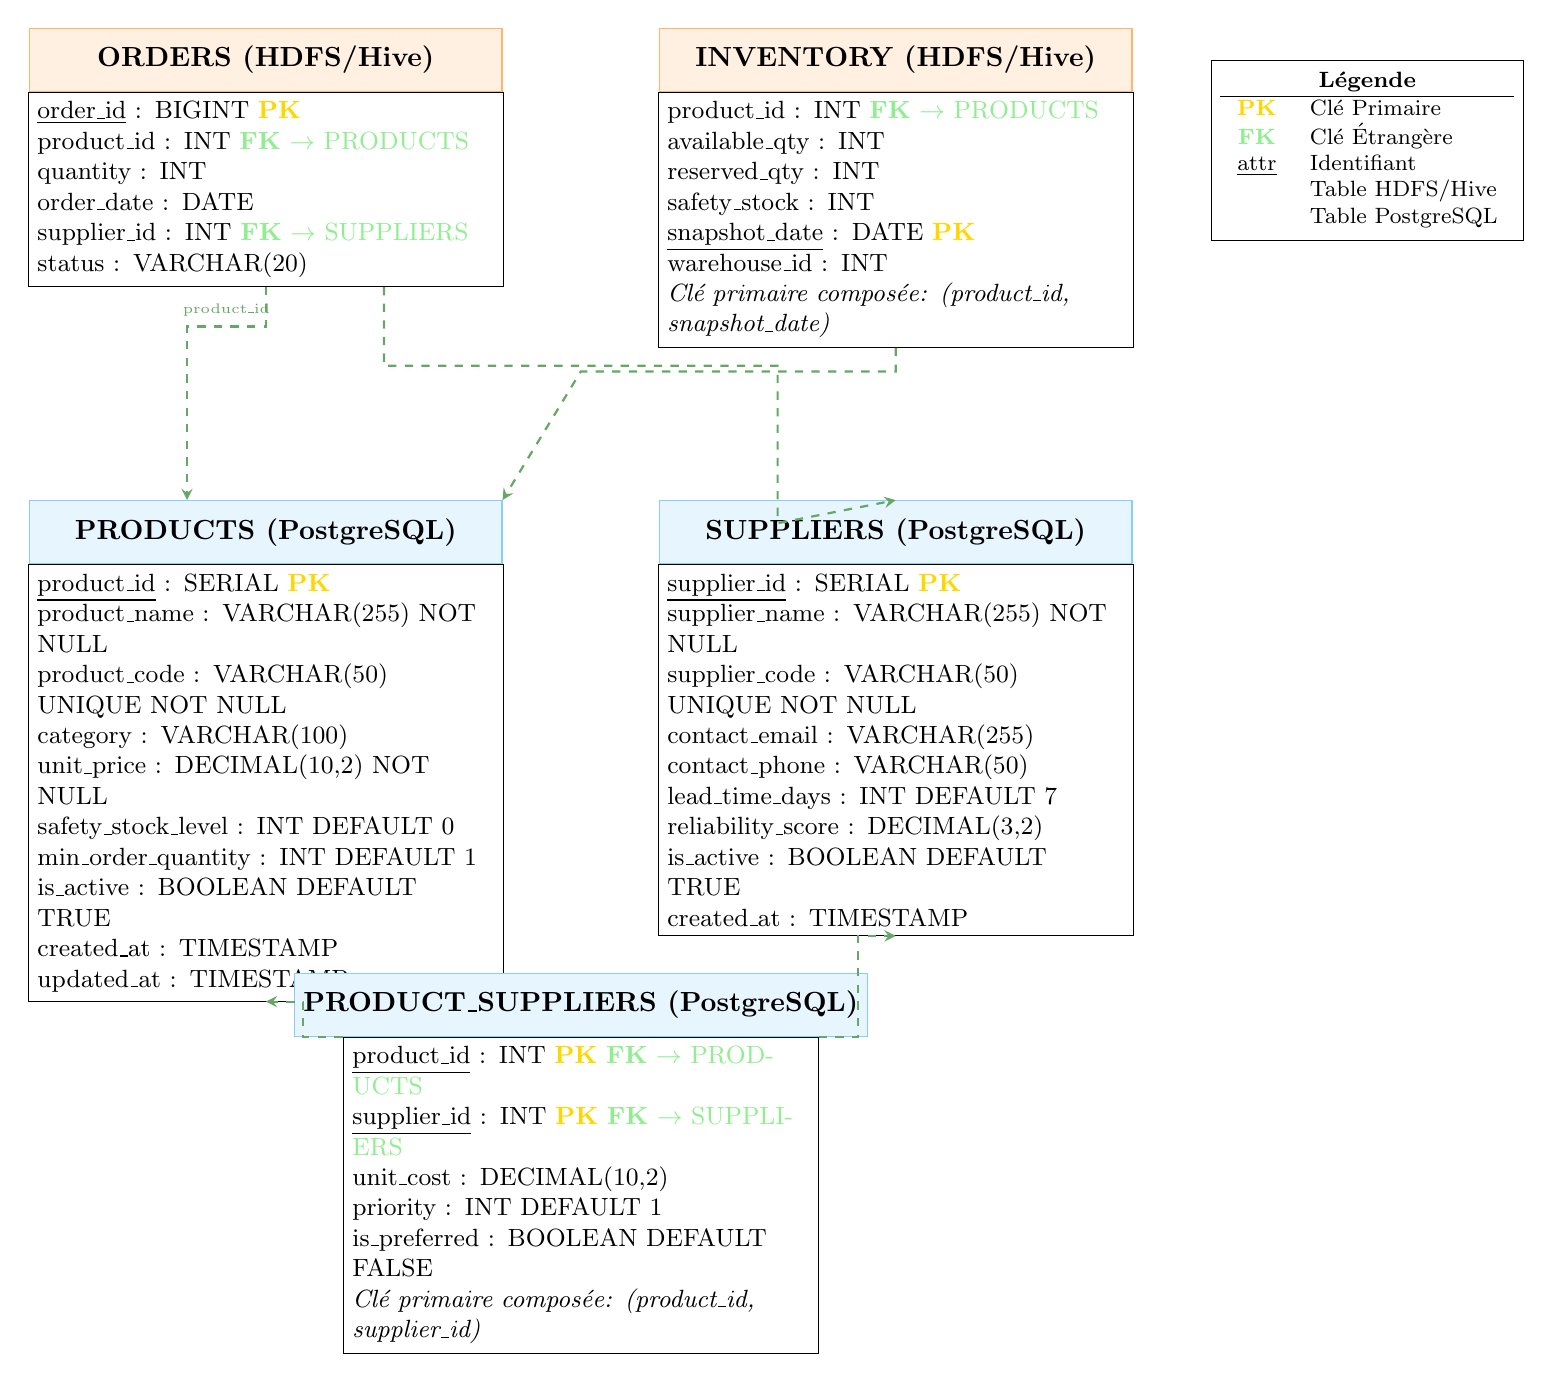
\begin{tikzpicture}[
    table/.style={
        rectangle, draw=black, fill=white,
        minimum width=6cm, text width=5.8cm,
        font=\small
    },
    tablename/.style={
        rectangle, draw=black, fill=primaryblue!30,
        minimum width=6cm, minimum height=0.8cm,
        font=\bfseries
    },
    hdfs/.style={
        rectangle, draw=hdfscolor, fill=hdfscolor!20,
        minimum width=6cm, minimum height=0.8cm,
        font=\bfseries
    },
    postgres/.style={
        rectangle, draw=postgrescolor, fill=postgrescolor!20,
        minimum width=6cm, minimum height=0.8cm,
        font=\bfseries
    },
    fkarrow/.style={->, >=stealth, thick, dashed, fkcolor!70!black}
]

% =====================================================
% HDFS TABLES
% =====================================================

% ORDERS Table
\node[hdfs] (orders_name) at (0, 10) {ORDERS (HDFS/Hive)};
\node[table, below=0pt of orders_name, anchor=north] (orders) {
    \underline{order\_id} : BIGINT \textcolor{pkcolor}{\textbf{PK}}\\
    product\_id : INT \textcolor{fkcolor}{\textbf{FK} $\rightarrow$ PRODUCTS}\\
    quantity : INT\\
    order\_date : DATE\\
    supplier\_id : INT \textcolor{fkcolor}{\textbf{FK} $\rightarrow$ SUPPLIERS}\\
    status : VARCHAR(20)
};

% INVENTORY Table
\node[hdfs] (inv_name) at (8, 10) {INVENTORY (HDFS/Hive)};
\node[table, below=0pt of inv_name, anchor=north] (inv) {
    product\_id : INT \textcolor{fkcolor}{\textbf{FK} $\rightarrow$ PRODUCTS}\\
    available\_qty : INT\\
    reserved\_qty : INT\\
    safety\_stock : INT\\
    \underline{snapshot\_date} : DATE \textcolor{pkcolor}{\textbf{PK}}\\
    warehouse\_id : INT\\
    \textit{Clé primaire composée: (product\_id, snapshot\_date)}
};

% =====================================================
% POSTGRESQL TABLES
% =====================================================

% PRODUCTS Table
\node[postgres] (prod_name) at (0, 4) {PRODUCTS (PostgreSQL)};
\node[table, below=0pt of prod_name, anchor=north] (prod) {
    \underline{product\_id} : SERIAL \textcolor{pkcolor}{\textbf{PK}}\\
    product\_name : VARCHAR(255) NOT NULL\\
    product\_code : VARCHAR(50) UNIQUE NOT NULL\\
    category : VARCHAR(100)\\
    unit\_price : DECIMAL(10,2) NOT NULL\\
    safety\_stock\_level : INT DEFAULT 0\\
    min\_order\_quantity : INT DEFAULT 1\\
    is\_active : BOOLEAN DEFAULT TRUE\\
    created\_at : TIMESTAMP\\
    updated\_at : TIMESTAMP
};

% SUPPLIERS Table
\node[postgres] (sup_name) at (8, 4) {SUPPLIERS (PostgreSQL)};
\node[table, below=0pt of sup_name, anchor=north] (sup) {
    \underline{supplier\_id} : SERIAL \textcolor{pkcolor}{\textbf{PK}}\\
    supplier\_name : VARCHAR(255) NOT NULL\\
    supplier\_code : VARCHAR(50) UNIQUE NOT NULL\\
    contact\_email : VARCHAR(255)\\
    contact\_phone : VARCHAR(50)\\
    lead\_time\_days : INT DEFAULT 7\\
    reliability\_score : DECIMAL(3,2)\\
    is\_active : BOOLEAN DEFAULT TRUE\\
    created\_at : TIMESTAMP
};

% PRODUCT_SUPPLIERS Table
\node[postgres] (ps_name) at (4, -2) {PRODUCT\_SUPPLIERS (PostgreSQL)};
\node[table, below=0pt of ps_name, anchor=north] (ps) {
    \underline{product\_id} : INT \textcolor{pkcolor}{\textbf{PK}} \textcolor{fkcolor}{\textbf{FK} $\rightarrow$ PRODUCTS}\\
    \underline{supplier\_id} : INT \textcolor{pkcolor}{\textbf{PK}} \textcolor{fkcolor}{\textbf{FK} $\rightarrow$ SUPPLIERS}\\
    unit\_cost : DECIMAL(10,2)\\
    priority : INT DEFAULT 1\\
    is\_preferred : BOOLEAN DEFAULT FALSE\\
    \textit{Clé primaire composée: (product\_id, supplier\_id)}
};

% =====================================================
% FOREIGN KEY ARROWS
% =====================================================

% Orders -> Products
\draw[fkarrow] (orders.south) -- ++(0,-0.5) -| node[pos=0.25, above, font=\tiny] {product\_id} ([xshift=-1cm]prod_name.north);

% Orders -> Suppliers
\draw[fkarrow] ([xshift=1.5cm]orders.south) -- ++(0,-1) -- ++(5,0) -- ++(0,-2) -- (sup_name.north);

% Inventory -> Products
\draw[fkarrow] (inv.south) -- ++(0,-0.3) -- ++(-4,0) -- (prod_name.north east);

% Product_Suppliers -> Products
\draw[fkarrow] (ps.north west) -- ++(-0.5,0) |- (prod.south);

% Product_Suppliers -> Suppliers
\draw[fkarrow] (ps.north east) -- ++(0.5,0) |- (sup.south);

% Legend
\node[draw, fill=white, font=\footnotesize, anchor=north west] at (12, 10) {
    \begin{tabular}{cl}
        \multicolumn{2}{c}{\textbf{Légende}}\\
        \hline
        \textcolor{pkcolor}{\textbf{PK}} & Clé Primaire\\
        \textcolor{fkcolor}{\textbf{FK}} & Clé Étrangère\\
        \underline{attr} & Identifiant\\
        \textcolor{hdfscolor}{$\blacksquare$} & Table HDFS/Hive\\
        \textcolor{postgrescolor}{$\blacksquare$} & Table PostgreSQL\\
    \end{tabular}
};

\end{tikzpicture}
}
\caption{MLD - Modèle Logique de Données}
\label{fig:mld}
\end{figure}

\subsection{Schema Notation}

The relational schema can also be represented in formal notation:

\begin{tcolorbox}[colback=white, colframe=primaryblue, title=\textbf{Schéma Relationnel}]

\textbf{HDFS/Hive Tables:}
\begin{itemize}
    \item \textbf{ORDERS} (\underline{order\_id}, product\_id\#, quantity, order\_date, supplier\_id\#, status)
    \item \textbf{INVENTORY} (\underline{product\_id\#, snapshot\_date}, available\_qty, reserved\_qty, safety\_stock, warehouse\_id)
\end{itemize}

\textbf{PostgreSQL Tables:}
\begin{itemize}
    \item \textbf{PRODUCTS} (\underline{product\_id}, product\_name, product\_code, category, unit\_price, safety\_stock\_level, min\_order\_quantity, is\_active, created\_at, updated\_at)
    \item \textbf{SUPPLIERS} (\underline{supplier\_id}, supplier\_name, supplier\_code, contact\_email, contact\_phone, lead\_time\_days, reliability\_score, is\_active, created\_at)
    \item \textbf{PRODUCT\_SUPPLIERS} (\underline{product\_id\#, supplier\_id\#}, unit\_cost, priority, is\_preferred)
\end{itemize}

\vspace{0.3cm}
\textit{Note: \underline{attribut} = clé primaire, attribut\# = clé étrangère}
\end{tcolorbox}

\newpage

% ============================================
% SECTION 4: DATA DICTIONARY
% ============================================
\section{Data Dictionary}

\subsection{ORDERS Table}

\begin{table}[H]
\centering
\begin{tabular}{|l|l|l|l|p{4cm}|}
\hline
\rowcolor{hdfscolor!50}
\textbf{Attribute} & \textbf{Type} & \textbf{Key} & \textbf{Nullable} & \textbf{Description} \\
\hline
order\_id & BIGINT & PK & NO & Unique order identifier \\
\hline
product\_id & INT & FK & NO & Reference to product \\
\hline
quantity & INT & - & NO & Ordered quantity \\
\hline
order\_date & DATE & Partition & NO & Date of order \\
\hline
supplier\_id & INT & FK & NO & Reference to supplier \\
\hline
status & VARCHAR(20) & - & YES & Order status (PENDING, etc.) \\
\hline
\end{tabular}
\caption{ORDERS - Data Dictionary}
\end{table}

\subsection{INVENTORY Table}

\begin{table}[H]
\centering
\begin{tabular}{|l|l|l|l|p{4cm}|}
\hline
\rowcolor{hdfscolor!50}
\textbf{Attribute} & \textbf{Type} & \textbf{Key} & \textbf{Nullable} & \textbf{Description} \\
\hline
product\_id & INT & PK, FK & NO & Reference to product \\
\hline
available\_qty & INT & - & NO & Available quantity \\
\hline
reserved\_qty & INT & - & NO & Reserved quantity \\
\hline
safety\_stock & INT & - & NO & Safety stock threshold \\
\hline
snapshot\_date & DATE & PK, Part & NO & Snapshot date \\
\hline
warehouse\_id & INT & - & YES & Warehouse identifier \\
\hline
\end{tabular}
\caption{INVENTORY - Data Dictionary}
\end{table}

\subsection{PRODUCTS Table}

\begin{table}[H]
\centering
\begin{tabular}{|l|l|l|l|p{4cm}|}
\hline
\rowcolor{postgrescolor!50}
\textbf{Attribute} & \textbf{Type} & \textbf{Key} & \textbf{Nullable} & \textbf{Description} \\
\hline
product\_id & SERIAL & PK & NO & Auto-increment ID \\
\hline
product\_name & VARCHAR(255) & - & NO & Product name \\
\hline
product\_code & VARCHAR(50) & UQ & NO & Unique product code \\
\hline
category & VARCHAR(100) & - & YES & Product category \\
\hline
unit\_price & DECIMAL(10,2) & - & NO & Unit selling price \\
\hline
safety\_stock\_level & INT & - & YES & Safety stock level \\
\hline
min\_order\_quantity & INT & - & YES & Minimum order qty \\
\hline
is\_active & BOOLEAN & - & YES & Active status \\
\hline
created\_at & TIMESTAMP & - & YES & Creation timestamp \\
\hline
updated\_at & TIMESTAMP & - & YES & Last update timestamp \\
\hline
\end{tabular}
\caption{PRODUCTS - Data Dictionary}
\end{table}

\subsection{SUPPLIERS Table}

\begin{table}[H]
\centering
\begin{tabular}{|l|l|l|l|p{4cm}|}
\hline
\rowcolor{postgrescolor!50}
\textbf{Attribute} & \textbf{Type} & \textbf{Key} & \textbf{Nullable} & \textbf{Description} \\
\hline
supplier\_id & SERIAL & PK & NO & Auto-increment ID \\
\hline
supplier\_name & VARCHAR(255) & - & NO & Supplier name \\
\hline
supplier\_code & VARCHAR(50) & UQ & NO & Unique supplier code \\
\hline
contact\_email & VARCHAR(255) & - & YES & Contact email \\
\hline
contact\_phone & VARCHAR(50) & - & YES & Contact phone \\
\hline
lead\_time\_days & INT & - & YES & Delivery lead time \\
\hline
reliability\_score & DECIMAL(3,2) & - & YES & Reliability score (0-1) \\
\hline
is\_active & BOOLEAN & - & YES & Active status \\
\hline
created\_at & TIMESTAMP & - & YES & Creation timestamp \\
\hline
\end{tabular}
\caption{SUPPLIERS - Data Dictionary}
\end{table}

\subsection{PRODUCT\_SUPPLIERS Table}

\begin{table}[H]
\centering
\begin{tabular}{|l|l|l|l|p{4cm}|}
\hline
\rowcolor{postgrescolor!50}
\textbf{Attribute} & \textbf{Type} & \textbf{Key} & \textbf{Nullable} & \textbf{Description} \\
\hline
product\_id & INT & PK, FK & NO & Reference to product \\
\hline
supplier\_id & INT & PK, FK & NO & Reference to supplier \\
\hline
unit\_cost & DECIMAL(10,2) & - & YES & Supplier's unit cost \\
\hline
priority & INT & - & YES & Supplier priority (1=best) \\
\hline
is\_preferred & BOOLEAN & - & YES & Preferred supplier flag \\
\hline
\end{tabular}
\caption{PRODUCT\_SUPPLIERS - Data Dictionary}
\end{table}

\newpage

% ============================================
% SECTION 5: FEDERATED QUERY ARCHITECTURE
% ============================================
\section{Federated Query Architecture}

\subsection{Data Flow Overview}

\begin{figure}[H]
\centering
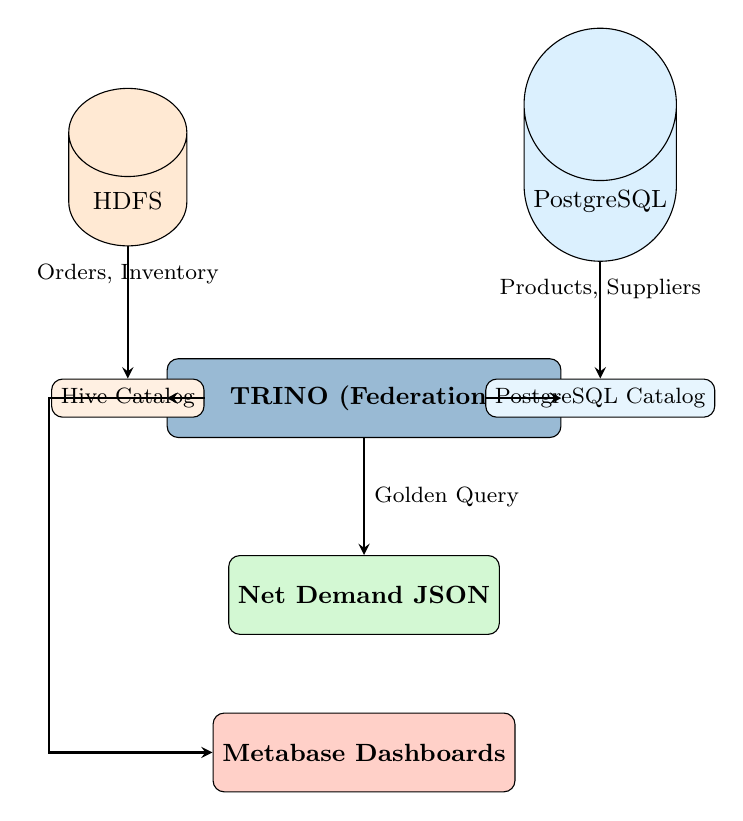
\begin{tikzpicture}[
    storage/.style={
        cylinder, draw, fill=white, shape border rotate=90,
        minimum height=2cm, minimum width=1.5cm, font=\small
    },
    process/.style={
        rectangle, draw, fill=primaryblue!20, rounded corners,
        minimum height=1cm, minimum width=3cm, font=\small\bfseries
    },
    arrow/.style={->, >=stealth, thick}
]

% Data Sources
\node[storage, fill=hdfscolor!30] (hdfs) at (0, 4) {HDFS};
\node[storage, fill=postgrescolor!30] (postgres) at (6, 4) {PostgreSQL};

% Labels
\node[below=0.1cm of hdfs, font=\footnotesize] {Orders, Inventory};
\node[below=0.1cm of postgres, font=\footnotesize] {Products, Suppliers};

% Trino
\node[process, fill=primaryblue!40, minimum width=5cm] (trino) at (3, 1.5) {TRINO (Federation)};

% Catalogs
\node[draw, fill=hdfscolor!20, font=\footnotesize, rounded corners] (hive_cat) at (0, 1.5) {Hive Catalog};
\node[draw, fill=postgrescolor!20, font=\footnotesize, rounded corners] (pg_cat) at (6, 1.5) {PostgreSQL Catalog};

% Output
\node[process, fill=fkcolor!40] (output) at (3, -1) {Net Demand JSON};

% Metabase
\node[process, fill=relationcolor!30] (metabase) at (3, -3) {Metabase Dashboards};

% Arrows
\draw[arrow] (hdfs) -- (hive_cat);
\draw[arrow] (postgres) -- (pg_cat);
\draw[arrow] (hive_cat) -- (trino);
\draw[arrow] (pg_cat) -- (trino);
\draw[arrow] (trino) -- node[right, font=\footnotesize] {Golden Query} (output);
\draw[arrow] (trino) -- ++(-4, 0) |- (metabase);

\end{tikzpicture}
\caption{Federated Query Architecture}
\label{fig:federation}
\end{figure}

\subsection{Golden Query - Net Demand Calculation}

The "Golden Query" performs a federated join across HDFS (Hive) and PostgreSQL data sources:

\begin{lstlisting}[language=SQL, caption={Net Demand Query}]
-- Federated Query via Trino
SELECT 
    p.product_id,
    p.product_name,
    p.safety_stock_level,
    i.available_qty,
    i.reserved_qty,
    COALESCE(SUM(o.quantity), 0) AS pending_orders,
    (i.available_qty - i.reserved_qty 
     - COALESCE(SUM(o.quantity), 0) 
     - p.safety_stock_level) AS net_demand,
    s.supplier_name,
    s.lead_time_days
FROM postgres.master_data.products p
JOIN hive.procurement_raw.inventory i 
    ON p.product_id = i.product_id
LEFT JOIN hive.procurement_raw.orders o 
    ON p.product_id = o.product_id 
    AND o.status = 'PENDING'
JOIN postgres.master_data.product_suppliers ps 
    ON p.product_id = ps.product_id 
    AND ps.is_preferred = TRUE
JOIN postgres.master_data.suppliers s 
    ON ps.supplier_id = s.supplier_id
WHERE i.snapshot_date = CURRENT_DATE
GROUP BY p.product_id, p.product_name, p.safety_stock_level,
         i.available_qty, i.reserved_qty, 
         s.supplier_name, s.lead_time_days
HAVING net_demand < 0
ORDER BY net_demand ASC;
\end{lstlisting}

\newpage

% ============================================
% SECTION 6: INDEXES AND CONSTRAINTS
% ============================================
\section{Indexes and Constraints}

\subsection{PostgreSQL Indexes}

\begin{table}[H]
\centering
\begin{tabular}{|l|l|l|p{4cm}|}
\hline
\rowcolor{primaryblue!20}
\textbf{Index Name} & \textbf{Table} & \textbf{Column(s)} & \textbf{Purpose} \\
\hline
idx\_products\_category & products & category & Filter by category \\
\hline
idx\_products\_active & products & is\_active & Filter active products \\
\hline
idx\_suppliers\_active & suppliers & is\_active & Filter active suppliers \\
\hline
idx\_ps\_priority & product\_suppliers & priority & Sort by priority \\
\hline
\end{tabular}
\caption{PostgreSQL Indexes}
\end{table}

\subsection{Hive Partitioning}

\begin{table}[H]
\centering
\begin{tabular}{|l|l|p{5cm}|}
\hline
\rowcolor{primaryblue!20}
\textbf{Table} & \textbf{Partition Column} & \textbf{Purpose} \\
\hline
orders & order\_date & Daily partition for efficient date filtering \\
\hline
inventory & snapshot\_date & Daily partition for snapshot isolation \\
\hline
\end{tabular}
\caption{Hive Partitioning Strategy}
\end{table}

\subsection{Referential Integrity Constraints}

\begin{table}[H]
\centering
\begin{tabular}{|l|l|l|}
\hline
\rowcolor{primaryblue!20}
\textbf{Constraint} & \textbf{Source} & \textbf{Target} \\
\hline
FK\_orders\_product & orders.product\_id & products.product\_id \\
\hline
FK\_orders\_supplier & orders.supplier\_id & suppliers.supplier\_id \\
\hline
FK\_inventory\_product & inventory.product\_id & products.product\_id \\
\hline
FK\_ps\_product & product\_suppliers.product\_id & products.product\_id \\
\hline
FK\_ps\_supplier & product\_suppliers.supplier\_id & suppliers.supplier\_id \\
\hline
\end{tabular}
\caption{Foreign Key Constraints}
\end{table}

\vspace{1cm}

\begin{center}
\textit{Note: Foreign key constraints between HDFS and PostgreSQL are enforced at the application level (Faker data generation) rather than at the database level due to the cross-system nature of the architecture.}
\end{center}

\end{document}
